\documentclass{ctexart}
\usepackage[utf8]{inputenc}
\usepackage{amsmath}
\usepackage{amsfonts}
\usepackage{amssymb}
\usepackage{listings}
\usepackage{graphicx}
\usepackage{float}

\title{CPU性能基准测试设计方案}
\author{张明昆2211585}
\date{\today}

\begin{document}

\maketitle

\begin{abstract}
本文档旨在介绍本小组设计的CPU性能的基准测试设计方案,通过一系列计算密集型任务,如质数计算、排序算法、矩阵运算和计算圆周率等,来评估CPU的处理速度。这些任务被设计为单线程执行,以测量CPU在单一核心上的性能。测试结果将基于每项任务完成所需的时间来评估CPU性能。
\end{abstract}

\section{背景}
在当今的计算环境中,CPU性能是衡量计算机整体性能的关键指标之一。随着计算需求的不断增长和多样化,从科学计算到日常应用,准确评估CPU性能变得至关重要。本测试集的设计目的是提供一种标准化的方法,通过执行一系列预定义的计算任务,来评估和比较不同CPU的性能。

\section{测试任务设计}
\subsection{质数计算}
质数计算通过筛选给定范围内的所有质数来评估CPU的性能。
在这里,我们使用了埃拉托斯特尼筛法(Sieve of Eratosthenes),这是一个高效的质数筛选算法。
该算法的基本思想是从2开始,将所有小于等于n的数的倍数标记为非质数(除了该数本身),剩下的未被标记的数即为质数。
这个过程要求CPU执行大量的除法和比较操作,能够有效地测试CPU处理简单重复任务的能力。
\begin{lstlisting}[language=C++]
    int primeCount(int n) {
        vector<bool> prime(n + 1, true);
        prime[0] = prime[1] = false;
        for (int p = 2; p * p <= n; p++) {
            if (prime[p]) {
                for (int i = p * p; i <= n; i += p) {
                    prime[i] = false;
                }
            }
        }
        return count(prime.begin(), prime.end(), true);
    }
\end{lstlisting}
\subsection{排序算法}
快速排序算法是一种高效的排序算法,采用分而治之的策略。
它首先选择一个“基准”值,然后将数组分成两部分,一部分包括所有小于基准的值,另一部分包括所有大于基准的值。
这个过程递归地在两个子数组上重复进行,直到整个数组排序完成。
\begin{lstlisting}[language=C++]
    void quickSort(vector<int>& arr, int left, int right) {
        int i = left, j = right;
        int pivot = arr[(left + right) / 2];
        while (i <= j) {
            while (arr[i] < pivot) i++;
            while (arr[j] > pivot) j--;
            if (i <= j) {
                swap(arr[i], arr[j]);
                i++;
                j--;
            }
        }
        if (left < j) quickSort(arr, left, j);
        if (i < right) quickSort(arr, i, right);
    }
\end{lstlisting}
\subsection{矩阵运算}
矩阵乘法是评估CPU执行复杂数学运算能力的一个重要指标。
该算法要求将两个矩阵A和B相乘,生成一个新的矩阵C。
对于矩阵C中的每个元素C[i][j],其值计算为矩阵A的第i行与矩阵B的第j列对应元素的乘积之和。
这个过程包含大量的乘法和加法操作,可以测试CPU处理复杂数学运算的能力。
\begin{lstlisting}[language=C++]
vector<vector<int>> matrixMultiply(const vector<vector<int>>& a,
                                   const vector<vector<int>>& b) {
    size_t n = a.size();
    vector<vector<int>> result(n, vector<int>(n, 0));
    for (size_t i = 0; i < n; i++) {
        for (size_t j = 0; j < n; j++) {
            for (size_t k = 0; k < n; k++) {
                result[i][j] += a[i][k] * b[k][j];
            }
        }
    }
    return result;
    }
\end{lstlisting}
\subsection{计算圆周率}
蒙特卡洛方法是一种统计模拟方法,用于计算圆周率π的值。
该方法通过随机生成点,并计算这些点落在单位圆内的比例来估计π值。
具体而言,算法生成大量随机点,并判断这些点是否位于单位圆内。
然后,根据单位圆内点的数量与总生成点的比例,利用公式4 * (单位圆内点的数量 / 总点数)来估计π值。
这个过程涉及到大量的随机数生成和数学运算,测试了CPU在处理随机性和计算密集型任务方面的性能。
\begin{lstlisting}[language=C++]
    double computePi(int samples) {
        default_random_engine gen;
        uniform_real_distribution<double> dist(0.0, 1.0);
        int count = 0;
        for (int i = 0; i < samples; i++) {
            double x = dist(gen);
            double y = dist(gen);
            if (x * x + y * y <= 1) count++;
        }
        return 4.0 * count / samples;
    }
\end{lstlisting}
\section{实现细节}
每项任务均设计为单线程执行,以便准确评估CPU在单核心上的性能。任务的规模被仔细选择,以确保每项任务的执行时间既不会太短,以致于难以测量,也不会太长,以免测试过程过于耗时。
为了确保测试结果的准确性和可重复性,每项任务都将重复执行多次,取平均值作为最终结果。
\section{测试流程}
\begin{enumerate}
    \item 准备阶段:在开始测试之前,确保测试环境稳定,关闭不必要的应用程序和后台进程,以减少对测试结果的干扰。
    \item 执行测试:依次执行每项计算任务,记录每项任务的完成时间。
    \item 结果分析:计算每项任务的平均完成时间。这些数据将用于评估CPU的性能。
\end{enumerate}
\section{测试结果}
通过在我们小组成员的电脑上运行该程序,并将测试结果经过python数据可视化后,我们绘制了以下图表。
\begin{figure}[H]
    \centering
    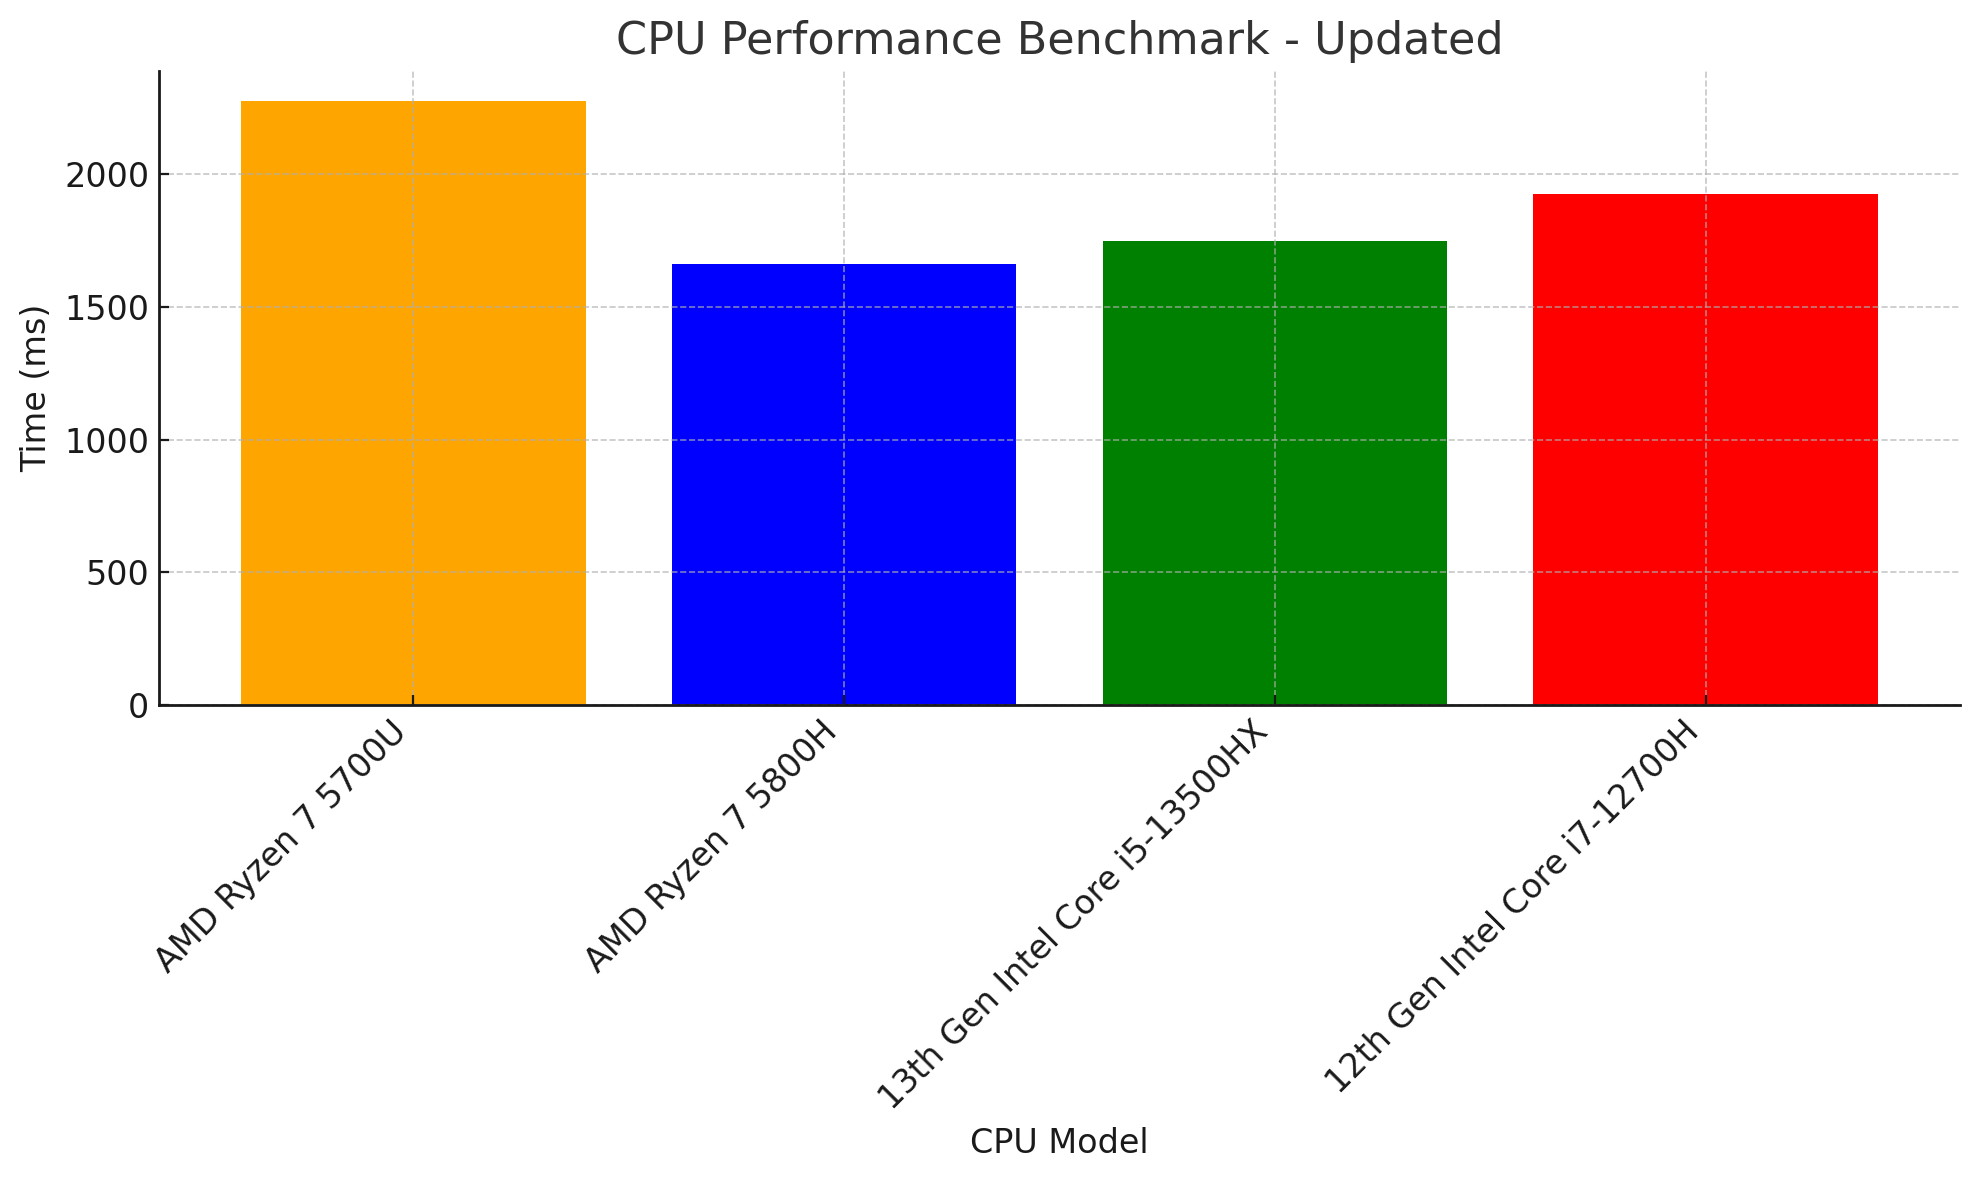
\includegraphics[width=1\textwidth]{3bae2083-77d4-4bf9-a107-23f6ebdfb357.png}
    \caption{CPU测试结果}
    \label{fig:image1}
    \end{figure}
\section{结论}
本文档提出的CPU性能基准测试设计方案,通过一系列计算任务,能够全面地评估CPU的处理速度。这种测试方法简单有效,易于实施。
通过这种方法,用户可以获得关于不同CPU性能的直观且实用的信息,为CPU的选择和性能优化提供科学依据。
\end{document}
